\begin{figure*}

\begin{subfigure}{\textwidth}
\begin{minipage}[b]{0.7265\textwidth}
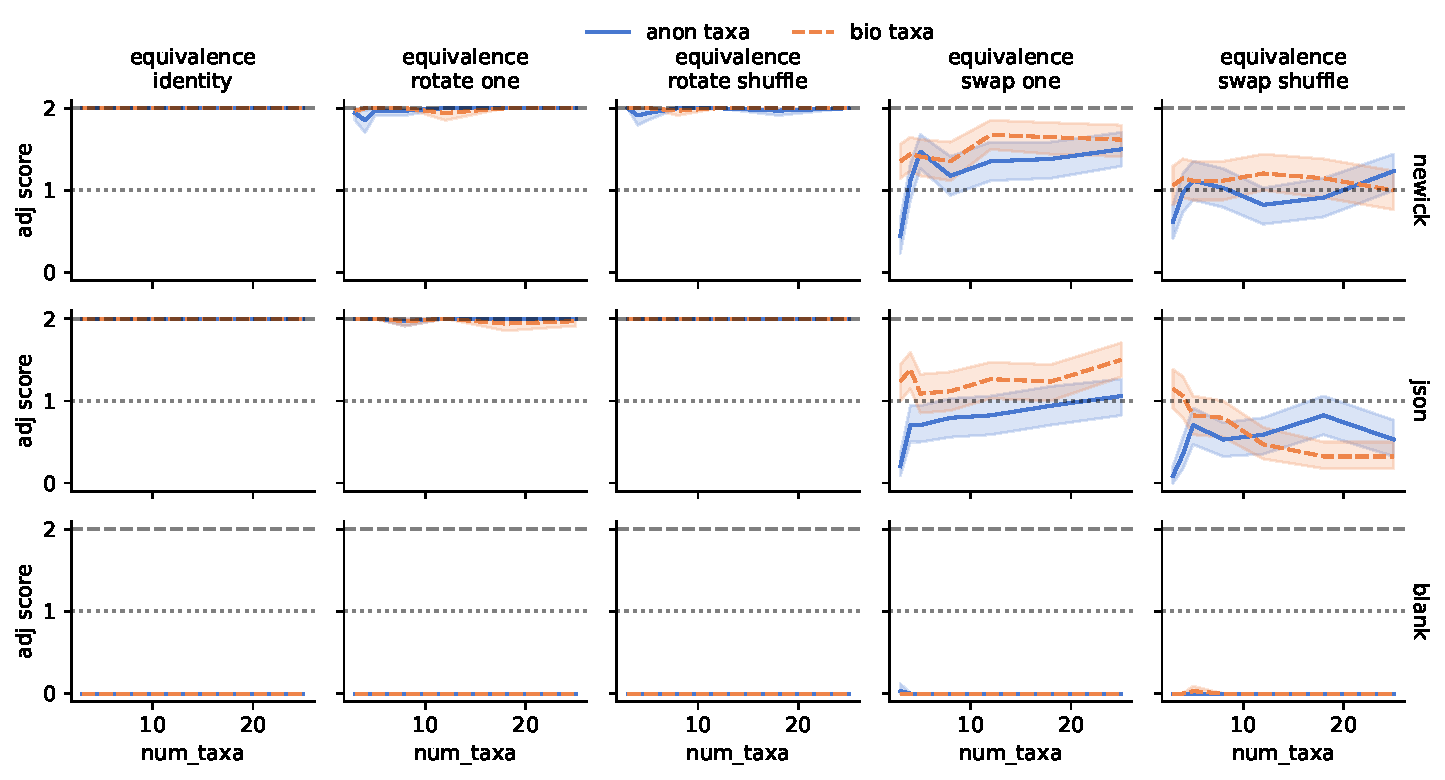
\includegraphics[width=\textwidth, trim={0cm 0cm 1cm 0.7cm}, clip]{binder/binder-2024-11-07-scientific.ipynb/binder/teeplots/2024-11-07-scientific/col=q+hue=tree-source+is_equivalence=True+kind=line+model=gpt-4o+palette=muted+row=tree-repr+style=tree-source+viz=relplot+x=num-taxa+y=adj-score+ext=.pdf}
\end{minipage}%
\begin{minipage}[b]{0.01\textwidth}
\end{minipage}
\begin{minipage}[b]{0.2635\textwidth}
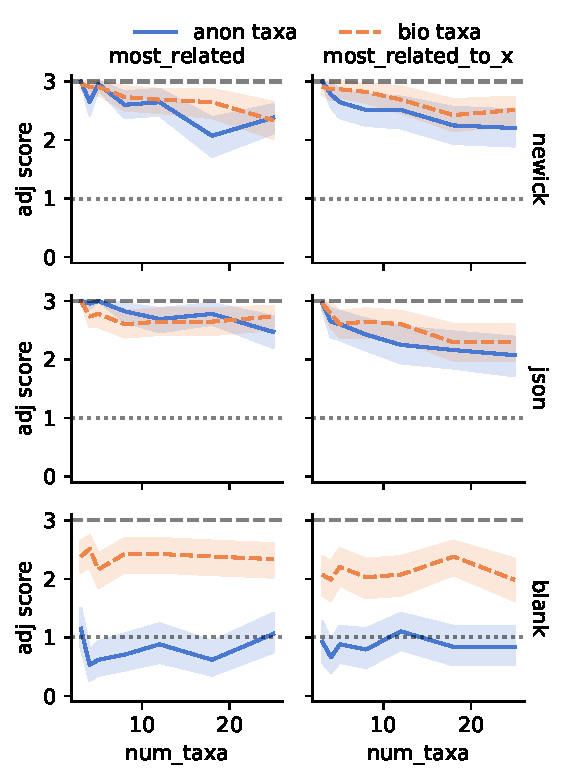
\includegraphics[width=\textwidth, trim={0.65cm 0cm 0cm 0cm}, clip]{binder/binder-2024-11-07-scientific.ipynb/binder/teeplots/2024-11-07-scientific/col=q+hue=tree-source+is_equivalence=False+kind=line+model=gpt-4o+palette=muted+row=tree-repr+style=tree-source+viz=relplot+x=num-taxa+y=adj-score+ext=.pdf}
\end{minipage}
\caption{gpt-4o}
\label{fig:taxatype:gpt-4o}
\end{subfigure}

\begin{subfigure}{\textwidth}
\begin{minipage}[b]{0.7265\textwidth}
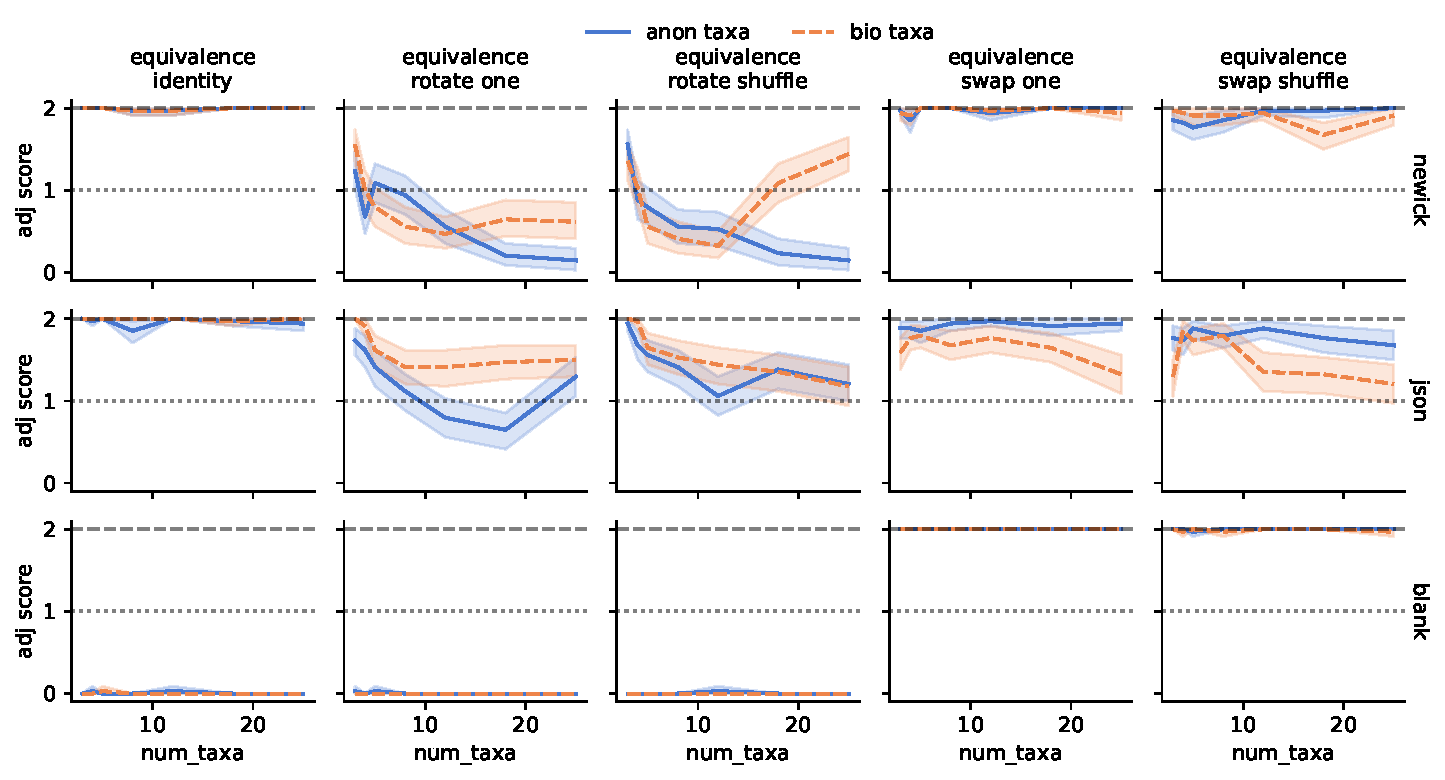
\includegraphics[width=\textwidth, trim={0cm 0cm 1cm 0.7cm}, clip]{binder/binder-2024-11-07-scientific.ipynb/binder/teeplots/2024-11-07-scientific/col=q+hue=tree-source+is_equivalence=True+kind=line+model=gpt-4o-mini+palette=muted+row=tree-repr+style=tree-source+viz=relplot+x=num-taxa+y=adj-score+ext=.pdf}
\end{minipage}%
\begin{minipage}[b]{0.01\textwidth}
\end{minipage}
\begin{minipage}[b]{0.2635\textwidth}
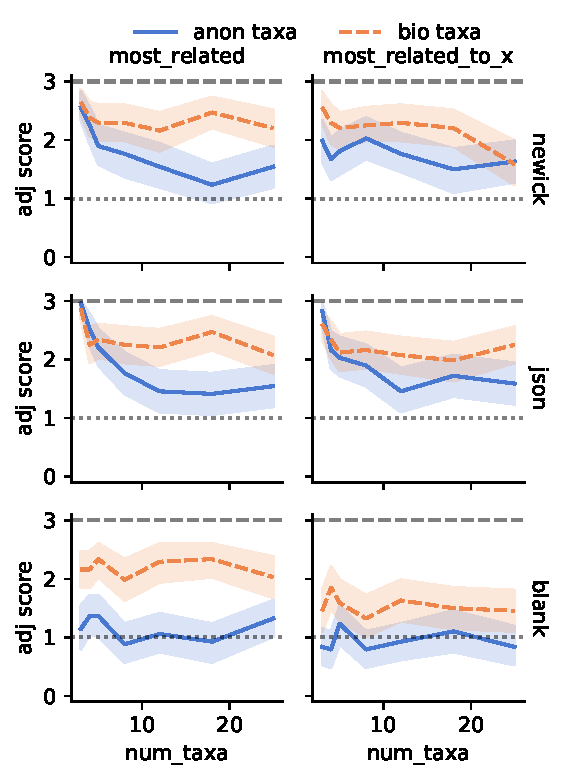
\includegraphics[width=\textwidth, trim={0.65cm 0cm 0cm 0cm}, clip]{binder/binder-2024-11-07-scientific.ipynb/binder/teeplots/2024-11-07-scientific/col=q+hue=tree-source+is_equivalence=False+kind=line+model=gpt-4o-mini+palette=muted+row=tree-repr+style=tree-source+viz=relplot+x=num-taxa+y=adj-score+ext=.pdf}
\end{minipage}
\caption{gpt-4o-mini}
\label{fig:taxatype:gpt-4o-mini}
\end{subfigure}

\caption{
\textbf{Taxa type comparison.}
Data from \citep{mammola2023biodiversity}.
Shaded bands denote bootstrapped 95\% CI, $n=100$.
}
\label{fig:taxatype}

\end{figure*}
